\begin{figure}[h]
    \centering
    
    % A
    \begin{subfigure}[b]{0.45\textwidth}
        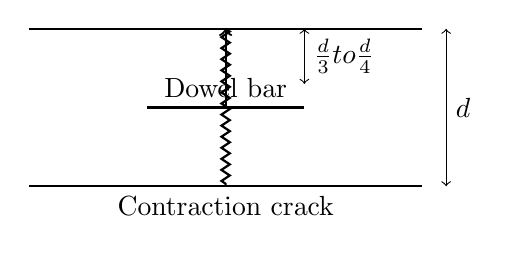
\begin{tikzpicture}
            % Outer Lines
            \draw[thick] (0,0) -- (5,0);
            \draw[thick] (0,2) -- (5,2);
            
            % Dowel Bar
            \draw[thick] (1.5,1) -- (3.5,1) node[midway, above] {Dowel bar};
            \draw[->, thick] (2.5,1) -- (2.5,2);
            
            % Dimension Lines
            \draw[<->] (5.3,0) -- (5.3,2) node[midway, right] {$d$};
            \draw[<->] (3.5,1.3) -- (3.5,2) node[midway, right] {$\frac{d}{3} \text{ to } \frac{d}{4}$};
            
            % Contraction Crack
            \draw[thick, decorate, decoration={zigzag, segment length=4, amplitude=1.5}] (2.5,2) -- (2.5,0) node[below] {Contraction crack};

		\label{A}
        \end{tikzpicture}

    \end{subfigure}
    \hfill
    % B
    \begin{subfigure}[b]{0.45\textwidth}
        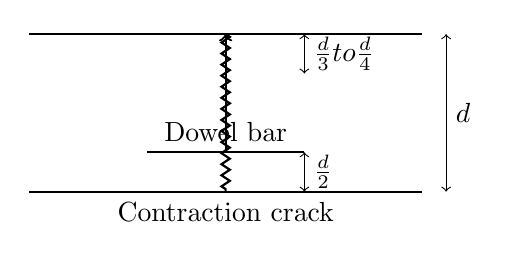
\begin{tikzpicture}
            % Outer Lines
            \draw[thick] (0,0) -- (5,0);
            \draw[thick] (0,2) -- (5,2);
            
            % Dowel Bar
            \draw[thick] (1.5,0.5) -- (3.5,0.5) node[midway, above] {Dowel bar};
            \draw[->, thick] (2.5,0.5) -- (2.5,2);
            
            % Dimension Lines
            \draw[<->] (5.3,0) -- (5.3,2) node[midway, right] {$d$};
            \draw[<->] (3.5,1.5) -- (3.5,2) node[midway, right] {$\frac{d}{3} \text{ to } \frac{d}{4}$};
            \draw[<->] (3.5,0) -- (3.5,0.5) node[midway, right] {$\frac{d}{2}$};
            
            % Contraction Crack
            \draw[thick, decorate, decoration={zigzag, segment length=4, amplitude=1.5}] (2.5,2) -- (2.5,0) node[below] {Contraction crack};
		\label{B}
        \end{tikzpicture}

    \end{subfigure}
    
    % C
    \begin{subfigure}[b]{0.45\textwidth}
        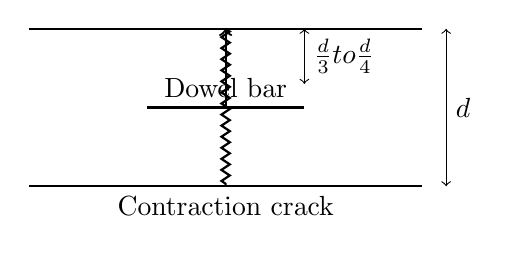
\begin{tikzpicture}
            % Outer Lines
            \draw[thick] (0,0) -- (5,0);
            \draw[thick] (0,2) -- (5,2);
            
            % Dowel Bar
            \draw[thick] (1.5,1) -- (3.5,1) node[midway, above] {Dowel bar};
            \draw[->, thick] (2.5,1) -- (2.5,2);
            
            % Dimension Lines
            \draw[<->] (5.3,0) -- (5.3,2) node[midway, right] {$d$};
            \draw[<->] (3.5,1.3) -- (3.5,2) node[midway, right] {$\frac{d}{3} \text{ to } \frac{d}{4}$};
            
            % Contraction Crack
            \draw[thick, decorate, decoration={zigzag, segment length=4, amplitude=1.5}] (2.5,2) -- (2.5,0) node[below] {Contraction crack};
		\label{C}
        \end{tikzpicture}

    \end{subfigure}
    \hfill
    % D
    \begin{subfigure}[b]{0.45\textwidth}
        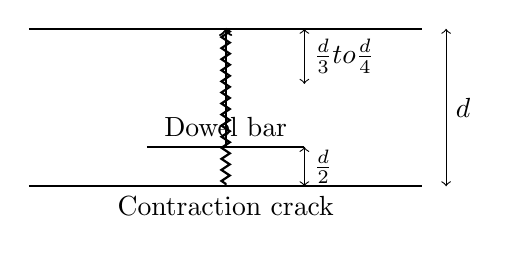
\begin{tikzpicture}
            % Outer Lines
            \draw[thick] (0,0) -- (5,0);
            \draw[thick] (0,2) -- (5,2);
            
            % Dowel Bar
            \draw[thick] (1.5,0.5) -- (3.5,0.5) node[midway, above] {Dowel bar};
            \draw[->, thick] (2.5,0.5) -- (2.5,2);
            
            % Dimension Lines
            \draw[<->] (5.3,0) -- (5.3,2) node[midway, right] {$d$};
            \draw[<->] (3.5,1.3) -- (3.5,2) node[midway, right] {$\frac{d}{3} \text{ to } \frac{d}{4}$};
            \draw[<->] (3.5,0) -- (3.5,0.5) node[midway, right] {$\frac{d}{2}$};
            
            % Contraction Crack
            \draw[thick, decorate, decoration={zigzag, segment length=4, amplitude=1.5}] (2.5,2) -- (2.5,0) node[below] {Contraction crack};
		\label{D}
        \end{tikzpicture}

    \end{subfigure}
    
   
\end{figure}


